\documentclass[a4paper]{amsart}
\usepackage[utf8]{inputenc}
\usepackage{enumerate}
\usepackage{url}
\usepackage{hyperref}

\usepackage{a4wide}
\theoremstyle{definition}
\newtheorem{task}{Úkol}


\title{\sc Cvičení z logiky: Domácí úkol č. 1}
%\author{Termín odevzdání: úterý 10. listopadu v 10:40}

\begin{document}


\medskip\begin{ukol}[2 body]
    {\it Před vypracováním si přečtěte pokyny popsané v podmínkách na zápočet!}
        
    \medskip    
        
    Adam, Barbora a Cyril jsou vyslýcháni, při jejich výslechu bylo zjištěno následující:
    \begin{itemize}\it
        \item Alespoň jeden z vyslýchaných říká pravdu a alespoň jeden lže.
        \item Adam říká: ``Barbora nebo Cyril lžou''
        \item Barbora říká: ``Cyril lže''
        \item Cyril říká: ``Adam nebo Barbora lžou''
    \end{itemize}
    \begin{enumerate}
        \item Vyjádřete naše znalosti jako výroky $\varphi_1$ až $\varphi_4$ nad množinou prvovýroků $\mathbb{P}=\{a,b,c\}$, přičemž $a,b,c$ znamená (po řadě), že {\it ``Adam/Barbora/Cyril říká pravdu''}.
        \item Najděte všechny modely teorie $T = \{\varphi_1, \dots, \varphi_4\}$.
        \item Najděte CNF teorii ekvivalentní teorii $T$.
        \item Ukažte (libovolnou metodou), že z teorie $T$ plyne, že: {\it Adam říká pravdu.}
    \end{enumerate}    
    \end{ukol}



    \medskip\begin{ukol}[2 body]{\,}
        \begin{enumerate}[label=\arabic*.]
            \item Převeďte následující výrok do CNF a DNF:
            $$
            ((p\to \neg q) \to \neg r) \to \neg p.
            $$
            \begin{enumerate}
                \item tabulkou (určením modelů),
                \item ekvivalentními úpravami (pokuste se najít co nejkratší CNF a DNF ekvivalenty).
            \end{enumerate}
            \item Uvažte  teorii $S=\{p_i \to (p_{i+1} \vee q_{i+1}), q_i \to (p_{i+1} \vee q_{i+1}) \mid i\in \mathbb{N}\}$ nad $\mathrm{var}(S)$.
            \begin{enumerate}
                    \item Které výroky ve tvaru  $p_i \to p_j$ jsou důsledky $S$?
                    \item Které výroky ve tvaru  $p_i \to (p_j \vee q_j)$ jsou důsledky $S$?
                    \item Určete všechny modely $S$.
            \end{enumerate}
        \end{enumerate} 
        \end{ukol}




        \medskip\begin{ukol}[3 body]{\,}
            \begin{enumerate}[label=\arabic*.]
            \item Pomocí algoritmu implikačního grafu najděte všechny modely následující teorie:
            $$
            T=\{p,\neg q \to \neg r,\neg q \to \neg s,r \to p,\neg s \to \neg p\}
            $$
            
            \item Pomocí algoritmu jednotkové propagace najděte všechny modely následující teorie:
            \begin{align*}
                &(\neg a \vee \neg b \vee c \vee \neg d)\wedge(\neg b \vee c)\wedge d \wedge (\neg a \vee \neg c \vee e)\wedge \\
                &(\neg c \vee \neg d)\wedge(\neg a \vee \neg d \vee \neg e)\wedge(a\vee \neg b \vee\neg e)
            \end{align*}
            
            \item Uvažme následující výroky $\varphi$ a $\psi$ nad $\mathbb P=\{p, q, r, s\}$:
            \begin{align*}
                \varphi &= (\neg p \vee  q)\to(p\wedge r)\\
                \psi &= s\to q
            \end{align*}
            \begin{enumerate}
                \item Určete počet (až na ekvivalenci) výroků $\chi$ nad $\mathbb P$ takových, že $\varphi\wedge\psi\models\chi$.
                \item Určete počet (až na ekvivalenci) úplných teorií $T$ nad $\mathbb P$ takových, že $T\models\varphi\wedge\psi$.
                \item Najděte nějakou axiomatizaci pro každou (až na ekvivalenci) kompletní teorii $T$ nad $\mathbb P$ takovou, že $T\models\varphi\wedge\psi$.
            \end{enumerate}
            \end{enumerate} 
            \end{ukol}


            \medskip\begin{ukol}[3 body]{\,}

                \begin{enumerate}[label=\arabic*.]
                \item Pomocí tablo metody:
                \begin{enumerate}
                    \item dokažte, že následující výrok je tautologie: 
                    $$(p \to (q \to r)) \to ((p\to q)\to (p \to r))$$
                    \item dokažte nebo najděte protipříklad ve formě \emph{kanonického} modelu pro bezespornou větev:
                    $$\{ p \to r,\ p \vee q,\ \neg s \to \neg q\} \models r \to s$$
                    \item určete všechny modely:
                    $$\{ q \to p,\ r \to q,\ (r \to p) \to s\}$$
                \end{enumerate}
                \item 
                \end{enumerate} 
                \end{ukol}



                \medskip\begin{ukol}[2 body]
                    Nechť $T$ je teorie jazyka $L=\langle T \rangle$ s rovností, kde $T$ je ternární relační symbol, s axiomy:
                    \begin{align*}
                        T(x,y,z)&\to x\ne y \wedge y\ne z \wedge x\ne z \\
                        T(x,y,z)&\to T(y,x,z)\wedge T(y,z,x)\wedge T(z,y,x)\wedge T(z,x,y)\wedge T(x,z,y)\\
                        x\ne y &\to (\exists z)(T(x,y,z)\wedge(\forall u)(T(x,y,u)\to u=z))
                    \end{align*}
                    Modely teorie $T$ jsou tzv. \emph{Steinerovy systémy trojic}, v našem případě uspořádaných. Uvažme model $\mathcal{F}=\langle \{1,2,\dots,7\},T^F\rangle$ teorie $T$ na obrázku (tzv. \emph{Fanova rovina}), kde každá ``přímka'' reprezentuje trojici prvků, jež jsou v relaci $T^F$ v libovolném pořadí, tedy $T^F=\{(2,4,6),(6,2,4),\dots\}$.
                    \begin{center}
                        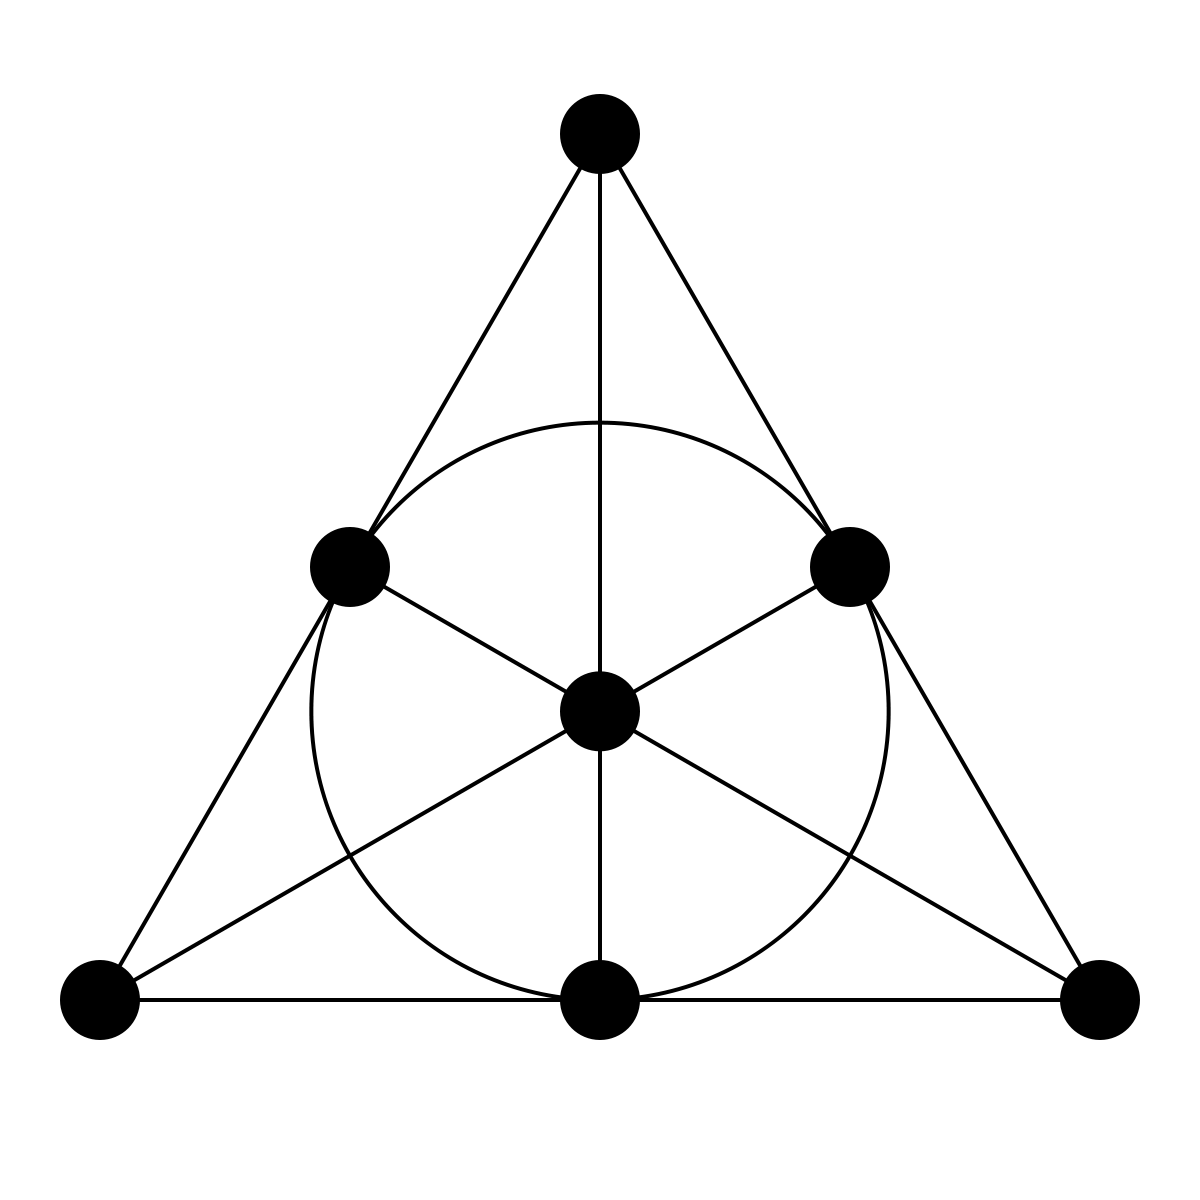
\includegraphics[height=4cm]{files/fano.png}  
                    \end{center}
                    \begin{enumerate}        
                        \item Nalezněte co nejmenší množinu parametrů $A$, která v modelu $\mathcal{F}$ umožňuje definovat libovolný jeho prvek (formulí jazyka $L$). Pro každý prvek napište příslušnou definující formuli (s dosazenými parametry). Zdůvodněte, proč je $A$ nejmenší možná.
                        \item Jsou teorie $T'=T \cup \{f(x,y)=z \leftrightarrow T(x,y,z)\}$ a $T''=T\cup \{f(x,y)=z \leftrightarrow T(x,y,z) \vee (x=y \wedge y=z)\}$, kde $f$ je nový binární funkční symbol, (korektními) extenzemi teorie $T$ o definici? Uveďte zdůvodnění.
                    \end{enumerate} 
                \end{ukol}


\maketitle

\thispagestyle{empty}

Úkol odevzdávejte v Moodle. Ponechte si dostatečný čas pro odevzdání, tak aby vám krátkodobé technické potíže s Moodle nezabránily úkol odevzdat. Pozdě odevzdané úkoly nebudou hodnoceny, kromě případů hodných zvláštního zřetele. Odevzdané řešení musí být vaše vlastní, není dovoleno hledat nápovědy ani řešení konzultovat s kýmkoliv kromě mne. Své odpovědi dostatečně podrobně zdůvodněte, uveďte všechny pomocné výpočty apod.


\begin{task}
Převeďte následující výrok do CNF a do DNF. (Uveďte celý postup, ne jen odpověď.)
$$
((p\to \neg q) \to \neg r) \vee \neg p.
$$
\end{task}

\begin{task}
Rozhodněte, zda je následující 2-CNF výrok splnitelný. Pokud ano, najděte nějaké splňující ohodnocení. Nakreslete příslušný implikační graf, a graf silně souvislých komponent v topologickém uspořádání.
\begin{align*}
&(a \vee  c) \wedge  (a \vee  \neg d) \wedge  (b \vee  \neg d) 
\wedge  (b \vee  \neg e) \wedge  (\neg c \vee  \neg e) 
\wedge  (\neg a \vee  \neg f)
\wedge \\ &\wedge (b\vee\neg c)\wedge
(\neg b \vee  f) \wedge  (c \vee  \neg f) \wedge \neg f
\end{align*}
\end{task}

\begin{task}
Rozhodněte, zda je následující výrok v Hornově tvaru splnitelný. Pokud ano, najděte nějaké splňující ohodnocení. (Uveďte celý postup, ne jen odpověď.)
\begin{align*}
&(\neg a \vee \neg b \vee c \vee \neg d)\wedge(\neg b \vee c)\wedge d \wedge (\neg a \vee \neg c \vee e)\wedge \\
&\wedge(\neg c \vee \neg d)\wedge(\neg a \vee \neg d \vee \neg e)\wedge(a\vee \neg b \vee\neg e)
\end{align*}
\end{task}

\begin{task}
Uvažme následující výroky $\varphi$ a $\psi$ nad $\mathbb P=\{p, q, r, s\}$:
\begin{align*}
    \varphi &= (\neg p \vee  q)\to(p\wedge r)\\
    \psi &= s\to q
\end{align*}
\begin{enumerate}[(a)]
    \item Určete počet (až na ekvivalenci) výroků $\chi$ nad $\mathbb P$ takových, že $\varphi\wedge\psi\models\chi$.
    \item Určete počet (až na ekvivalenci) úplných teorií $T$ nad $\mathbb P$ takových, že $T\models\varphi\wedge\psi$.
    \item Najděte nějakou axiomatizaci pro každou (až na ekvivalenci) úplnou teorii $T$ nad $\mathbb P$ takovou, že $T\models\varphi\wedge\psi$.
\end{enumerate}


\end{task}


\begin{task}
Uvažme následující tvrzení:
\begin{enumerate}
\item[$(i)$] {\it Ten, kdo je dobrý běžec a má dobrou kondici, uběhne maraton.}
\item[$(ii)$] {\it Ten, kdo nemá štěstí a nemá dobrou kondici, neuběhne maraton.}
\item[$(iii)$]{\it Ten, kdo uběhne maraton, je dobrý běžec.}
\item[$(iv)$] {\it Budu-li mít štěstí, uběhnu maraton.}
\item[$(v)$] {\it Mám dobrou kondici.}
\end{enumerate}


\begin{enumerate}[(a)]
\item Přeložte tvrzení (i) až (v) po řadě do výroků $\varphi_1$ až $\varphi_5$ v jazyce $L=\langle b, k, m, s\rangle$, kde výrokové proměnné mají po řadě význam ``být dobrý běžec'', ``mít dobrou kondici'', ``uběhnout maraton'' a ``mít štěstí''.
\item Sestrojte dokončené tablo z teorie $T=\{\varphi_1,\dots,\varphi_5\}$ s položkou $F (k \wedge \neg k)$ v kořeni. Sestrojte kanonický model pro nejlevější bezespornou větev tohoto tabla.

\item Najděte příklad výroků v jazyce $L$, které jsou $T$-ekvivalentní, ale ne logicky ekvivalentní. 
\item Určete počet navzájem neekvivalentních jednoduchých extenzí teorie $T$.
\end{enumerate}
\end{task}



\end{document}
